\documentclass[10pt]{article}
\usepackage{icmlko}

\icmlmeta{IP 파운데이션 월드모델}{57}{검정에서 진 쪽이 대체재였다}{반증 조건을 걸었더니 내 설명이 틀렸다 --- 그리고 공통 축의 최적 변수와 고유 축의 최적 변수가 다르다}

\begin{document}

\twocolumn[
\icmlheader

\begin{abstract}
노트 56은 웹툰에서 타깃 폭을 끄면 고유 축이 $+$0.0458로 크게 회복하는 것을
보고 ``고유 축에 태그 수가 있고 그것이 원래 타깃 폭이었기 때문''이라고 읽었다.
반증 조건도 적었다 --- ``태그 수를 고유 축에서 빼고 다시 재면 검정된다.''
\textbf{틀렸다.} 태그 수를 빼도 회복이 $+$0.0420으로 거의 그대로이고,
\textbf{연령 등급}을 빼면 $-$0.0311로 사라진다. 회복을 만드는 것은 연령
등급이었다 --- 노트 46에서 타깃 폭 자리를 놓고 태그 수에 \emph{진} 변수다.
그렇다면 함의가 있다. 공통 축으로 넣을 때와 고유 축으로 넣을 때 최적 변수가
다를 수 있다는 것이다. 직접 쟀다. \textbf{고유 축이 없으면 태그 수를 공통으로
쓰는 쪽이 낫고($+$0.3440 대 $+$0.3388), 고유 축이 있으면 연령 등급을 공통으로
쓰는 쪽이 낫다($+$0.3485 대 $+$0.3327).} 순서가 뒤집힌다. 이유는 두 자리의
역할이 다르기 때문이다 --- 공통 축은 프로크루스테스 정렬에 참여하므로 도메인
간 대응이 중요하고, 고유 축은 정렬에 불참하고 인자 공간에만 기여하므로 그
도메인 안에서의 설명력이 중요하다. 다만 뒤집힌 쪽의 짝지은 구간이
{[}$-$0.148, $+$0.041{]}로 매우 넓어(P$=$0.553) \textbf{채택하지 않았다}.
실무 교훈은 남는다 --- \textbf{배선은 공통/고유 배치와 함께 정해야 하고 슬롯
단위로 따로 최적화하면 안 된다.}
\end{abstract}
]

\section{반증 조건이 발동했다}

노트 56의 설명은 이랬다 --- 웹툰 타깃 폭을 끄면 고유 축이 $+$0.0458 회복하는데,
고유 축에 태그 수가 있고 그것이 원래 타깃 폭이었기 때문이다. 그리고 검정 방법을
같이 적었다.

\begin{figure}[t]
\centering
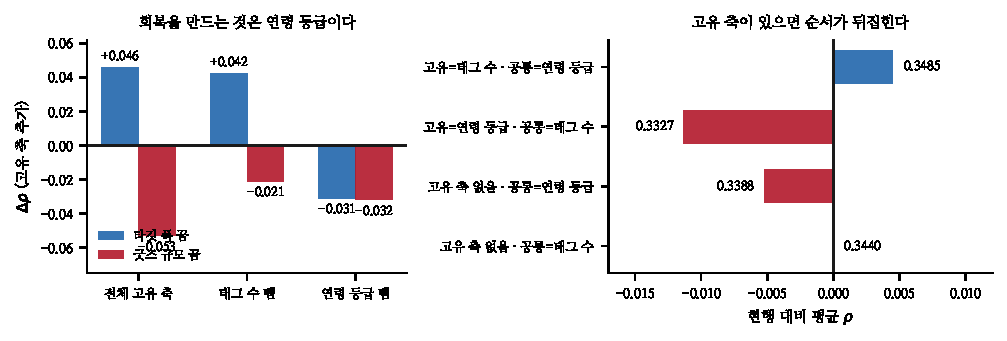
\includegraphics[width=\textwidth]{figs/swap.pdf}
\caption{왼쪽 --- 고유 축에서 하나씩 뺄 때. 오른쪽 --- 네 배치의 비교.}
\end{figure}

\begin{table}[t]
\centering\tsize
\caption{웹툰 고유 축에서 하나씩 빼고 다시 잰 것.}
\begin{tabular}{lrr}
\toprule
고유 축 구성 & 타깃 폭 끔 & 굿즈 규모 끔 \\
\midrule
전체(연령·태그·회차·요일) & $+$0.0458 & $-$0.0530 \\
태그 수 뺌 & \textbf{$+$0.0420} & $-$0.0209 \\
연령 등급 뺌 & \textbf{$-$0.0311} & $-$0.0320 \\
\bottomrule
\end{tabular}
\end{table}

태그 수를 빼도 회복이 거의 그대로다. \textbf{연령 등급을 빼면 사라지고 부호까지
뒤집힌다.} 내 설명이 지목한 변수가 아니었다.

\claimx{노트 56의 ``태그 수가 타깃 폭을 대신한다''를 철회한다. 대신하는 것은
연령 등급이며, 그것은 노트 46에서 타깃 폭 자리를 놓고 태그 수에 진 변수다.}
{연령 등급이 회복을 만드는 이유를 아직 모른다. 다른 도메인에서 ``진 쪽이 고유
축으로는 낫다''가 재현되어야 규칙이라 할 수 있다.}

\section{그러면 최적 변수가 자리마다 다른가}

노트 46은 태그 수와 연령 등급을 \emph{공통 축} 자리에서만 비교했다. 고유 축이
없는 상태였다. 고유 축을 함께 두고 다시 비교했다.

\begin{table}[t]
\centering\tsize
\caption{웹툰 타깃 폭 자리의 네 배치.}
\begin{tabular}{lr}
\toprule
배치 & 평균 $\rho$ \\
\midrule
\multicolumn{2}{l}{\emph{고유 축 없음}} \\
\quad 공통 $=$ 태그 수 (현행) & \textbf{$+$0.3440} \\
\quad 공통 $=$ 연령 등급 & $+$0.3388 \\
\midrule
\multicolumn{2}{l}{\emph{고유 축 있음}} \\
\quad 공통 $=$ 태그 수, 고유에 연령 등급 & $+$0.3327 \\
\quad 공통 $=$ 연령 등급, 고유에 태그 수 & \textbf{$+$0.3485} \\
\bottomrule
\end{tabular}
\end{table}

\textbf{순서가 뒤집힌다.} 고유 축이 없으면 태그 수가 $+$0.0052 앞서고, 있으면
연령 등급이 $+$0.0158 앞선다.

\claimx{공통 축의 최적 변수와 고유 축의 최적 변수가 다를 수 있다. 공통 축은
정렬에 참여하므로 도메인 간 대응이 중요하고, 고유 축은 정렬에 불참하고 인자
공간에만 기여하므로 그 도메인 안에서의 설명력이 중요하다.}{짝지은 구간이
$[-0.148,\ +0.041]$로 매우 넓다(P$=$0.553). 점추정의 역전이지 확인된 것이
아니다.}

\paragraph{채택하지 않았다}
$+$0.3485가 현행 $+$0.3440보다 높지만 구간이 0을 크게 포함한다. 노트 44 이후로
지켜 온 기준대로 보류한다.

\section{그래도 남는 교훈}

\begin{quote}\fontsize{9.5}{11.5}\selectfont
지금까지 배선 탐색을 \textbf{슬롯 단위}로 했다 --- 이 슬롯에 어느 변수를 넣을
것인가. 그런데 답이 고유 축의 존재 여부에 달려 있다면 슬롯 단위 최적화는
지역 최적만 찾는다. \textbf{배선은 공통/고유 배치와 함께 정해야 한다.}
\end{quote}

이것이 노트 45와 49의 ``배선 소진''을 다시 보게 만든다. 두 노트 모두 슬롯
단위로 후보를 훑었다 --- 여섯 도메인 63개 후보에서 문턱 통과가 0개였다. 공통과
고유를 함께 움직이는 탐색은 아직 하지 않았고, 그 공간은 훨씬 넓다.

다만 그 탐색은 후보 수가 곱으로 늘어 선택 편향이 커진다. 지금 구간 반폭이
0.056인데 그 안에서 수백 개를 훑으면 노트 44가 경고한 상황이 그대로 재현된다.

\section{한계}

\begin{itemize}[leftmargin=1.1em,itemsep=0.15em]
\item 역전을 웹툰 한 도메인, 한 슬롯에서만 봤다.
\item 구간이 $[-0.148,\ +0.041]$로 너무 넓어 사실상 아무것도 배제하지 못한다.
      150회로 돌렸는데 회수를 늘려도 폭이 크게 줄지는 않을 것이다.
\item 연령 등급이 왜 고유 축으로 더 나은지 모른다. 두 변수의 상관도 안 봤다.
\item 웹툰이 1,141건까지 수집됐는데 이 실험은 900건 상태 기준이다.
\item ``공통/고유를 함께 움직이는 탐색''을 제안만 하고 하지 않았다. 선택 편향
      때문에 지금 표본에서는 하지 않는 것이 맞다고 보았다.
\end{itemize}

\section{다음}

\begin{enumerate}[leftmargin=1.3em,itemsep=0.15em]
\item 웹툰 전체 수집 완료 후 전면 재측정 --- 구간이 좁아지면 이 역전을 다시
      판정할 수 있다.
\item 다른 도메인에서 ``진 쪽이 고유 축으로 낫다''가 재현되는지.
\item 태그 수와 연령 등급의 상관 --- 둘이 겹치면 배치 문제가 아니라 중복 문제다.
\item 공통/고유 결합 탐색의 선택 편향을 계산해 둔다. 언제 해도 되는지 미리
      정해 두는 편이 낫다.
\end{enumerate}

\vspace{0.6em}
\hrule height 0.3pt
\vspace{0.5em}
{\footnotesize
\textbf{참고문헌}\\[0.3em]
Meredith, W. (1993). Measurement invariance, factor analysis and factorial
invariance. \emph{Psychometrika}, 58(4), 525--543.\\[0.15em]
Schönemann, P. H. (1966). A generalized solution of the orthogonal Procrustes
problem. \emph{Psychometrika}, 31(1), 1--10.\\[0.15em]
Cawley, G. C., Talbot, N. L. C. (2010). On over-fitting in model selection and
subsequent selection bias in performance evaluation. \emph{JMLR}, 11, 2079--2107.\\[0.15em]
Guyon, I., Elisseeff, A. (2003). An introduction to variable and feature selection.
\emph{JMLR}, 3, 1157--1182.\\[0.15em]
Ben-David, S. et al. (2010). A theory of learning from different domains.
\emph{Machine Learning}, 79(1--2), 151--175.
}

\end{document}
